\section{Questao 4 - CSP e Otimizacoes de Busca}

\subsection{Modelagem do CSP}
\[
P=\langle X,D,C \rangle
\]
\begin{itemize}[leftmargin=1.5em]
  \item Variaveis: $X=\{T_1,T_2,T_3,T_4,T_5,T_6\}$.
  \item Dominio: $D(T_i)=\{A,B,C,D\}$ para todo $i$.
  \item Restricoes unarias: $T_2 \neq A$ e $T_5 \neq A$.
  \item Restricoes binarias:
  \[
  T_i \neq T_{i+1}, \quad i=1,\dots,5
  \]
  e a restricao adicional $((T_2=C)\land(T_5=C))$ proibida.
  \item Restricoes globais:
  \begin{itemize}[leftmargin=1.5em]
    \item $B$ deve aparecer em pelo menos um entre $T_3$ ou $T_4$;
    \item medico $D$ pode aparecer no maximo 2 vezes na escala.
  \end{itemize}
\end{itemize}

\subsection{Grafo de restricoes}
\begin{figure}[H]
\centering
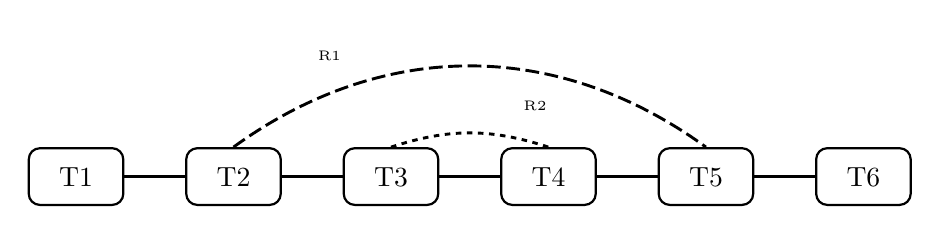
\begin{tikzpicture}[
  every node/.style={draw, rounded corners, minimum width=1.2cm, minimum height=0.72cm},
  every path/.style={thick},
  solidc/.style={black},
  extracA/.style={black, line width=1.05pt, dash pattern=on 5pt off 2pt},
  extracB/.style={black, line width=1.05pt, dash pattern=on 2pt off 2pt},
  edgelabel/.style={draw=none, fill=none, font=\tiny, inner sep=0.4pt}
]
\node (t1) at (0,0) {T1};
\node (t2) at (2,0) {T2};
\node (t3) at (4,0) {T3};
\node (t4) at (6,0) {T4};
\node (t5) at (8,0) {T5};
\node (t6) at (10,0) {T6};

\draw[solidc] (t1) -- (t2);
\draw[solidc] (t2) -- (t3);
\draw[solidc] (t3) -- (t4);
\draw[solidc] (t4) -- (t5);
\draw[solidc] (t5) -- (t6);
\draw[extracA] (t2.north) to[bend left=36] node[edgelabel, pos=0.22, above=2pt, xshift=-2pt] {R1} (t5.north);
\draw[extracB] (t3.north) to[bend left=18] node[edgelabel, pos=0.82, above=1pt, xshift=6pt] {R2} (t4.north);
\end{tikzpicture}
\vspace{0.1cm}

\begin{minipage}{0.92\linewidth}
\footnotesize
\textbf{Legenda:} arestas solidas representam $T_i \neq T_{i+1}$; \quad
R1: $\neg(T_2=C \land T_5=C)$; \quad
R2: cobertura de $B$ em $(T_3,T_4)$.
\end{minipage}
\caption{Grafo de restricoes usado na implementacao}
\end{figure}

\subsection{Backtracking (manual + implementado)}
Ordem fixa de atribuicao: $T_1 \rightarrow T_2 \rightarrow T_3 \rightarrow T_4 \rightarrow T_5 \rightarrow T_6$.

\begingroup
\small
\setlength{\tabcolsep}{5pt}
\renewcommand{\arraystretch}{1.08}
\begin{longtable}{c c >{\raggedright\arraybackslash}p{6.2cm} c}
\toprule
Passo & Tentativa & Estado parcial & Resultado \\
\midrule
1 & $T_1=A$ & \small $\{T_1=A\}$ & segue \\
2 & $T_2=B$ & \small $\{T_1=A,T_2=B\}$ & segue \\
3 & $T_3=A$ & \small $\{T_1=A,T_2=B,T_3=A\}$ & segue \\
4 & $T_4=A$ & \small $\{T_1=A,T_2=B,T_3=A,T_4=A\}$ & conflito \\
5 & $T_4=B$ & \small $\{T_1=A,T_2=B,T_3=A,T_4=B\}$ & segue \\
6 & $T_5=B$ & \small $\{T_1=A,T_2=B,T_3=A,T_4=B,T_5=B\}$ & conflito \\
7 & $T_5=C$ & \small $\{T_1=A,T_2=B,T_3=A,T_4=B,T_5=C\}$ & segue \\
8 & $T_6=A$ & \small $\{T_1=A,T_2=B,T_3=A,T_4=B,T_5=C,T_6=A\}$ & solucao \\
\bottomrule
\end{longtable}
\endgroup

\textbf{Estado final encontrado:} $(A,B,A,B,C,A)$.

\subsection{MRV + Degree}
Com MRV (e desempate por Degree), a busca inicia por variaveis mais restritas ($T_2$, $T_5$). Nesta instancia, essa estrategia aumentou o numero de estados explorados em relacao ao BT de ordem fixa, mas ainda encontra a mesma solucao final.

\subsection{Forward Checking}
O Forward Checking elimina valores inviaveis de dominios assim que uma atribuicao e feita. Nos primeiros passos da execucao:

\begingroup
\footnotesize
\setlength{\tabcolsep}{3pt}
\renewcommand{\arraystretch}{1.08}
\begin{longtable}{c c >{\raggedright\arraybackslash}p{5.25cm} >{\raggedright\arraybackslash}p{2.65cm}}
\toprule
Passo & Atribuicao & Dominios removidos/reduzidos & Observacao \\
\midrule
1 & $T_2=B$ & remove $B$ de $T_1$ e $T_3$ & restricao de consecutividade \\
2 & $T_5=B$ & remove $B$ de $T_4$ e $T_6$ & restricao de consecutividade \\
3 & $T_3=A$ & cobertura de $B$ forca $T_4=\{B\}$, mas $B$ ja removido de $T_4$ & dominio vazio em $T_4$ (inconsistencia) \\
4 & $T_3=C$ & mesma poda do passo 3 & inconsistencia \\
5 & $T_3=D$ & mesma poda do passo 3 & inconsistencia \\
6 & troca para $T_5=C$ & libera consistencia para $T_3$ e $T_4$ & busca volta a crescer \\
7--10 & $T_3=A,T_4=B,T_1=A,T_6=A$ & apenas podas locais de consecutividade & solucao encontrada \\
\bottomrule
\end{longtable}
\endgroup

Com isso, o FC detecta inconsistencias mais cedo e evita explorar subarvores inteiras que o BT simples ainda visitaria.

\subsection{Backjumping}
Nesta instancia, o Backjumping encontrou a solucao com o mesmo numero de estados do BT fixo e sem salto longo (saltos BJ = 0). Os conflitos identificados foram:
\begin{itemize}[leftmargin=1.5em]
  \item $T_4=A$ conflita com $T_3=A$ (restricao de consecutividade);
  \item $T_5=B$ conflita com $T_4=B$ (restricao de consecutividade).
\end{itemize}
Como os conflitos foram sempre com a variavel pai imediata, nao houve oportunidade de backjump para ancestrais mais altos.

\subsection{Comparacao quantitativa (Q4)}
\textbf{Todas as abordagens encontraram a mesma solucao:} $(A,B,A,B,C,A)$.
\begin{table}[H]
\centering
\begingroup
\footnotesize
\begin{tabular}{l c c c c c}
\toprule
Criterio & BT & BT+MRV & BT+MRV+Degree & FC & BJ \\
\midrule
Estados explorados & 8 & 59 & 59 & 10 & 8 \\
Backtracks & 0 & 13 & 13 & 1 & 0 \\
Profundidade maxima & 6 & 6 & 6 & 6 & 6 \\
Saltos BJ & 0 & 0 & 0 & 0 & 0 \\
\bottomrule
\end{tabular}
\endgroup
\caption{Resultados medidos pela implementacao autoral}
\end{table}

\subsection{Analise final pedida na questao}
\begin{itemize}[leftmargin=1.5em]
  \item Numero de estados explorados: melhor resultado em BT e BJ (8), seguido de FC (10).
  \item Numero de retrocessos: BT/BJ (0), FC (1), MRV e MRV+Degree (13).
  \item Velocidade de execucao: para esta instancia pequena, BT/BJ e FC foram mais rapidos.
  \item Consumo de memoria: todos baixos; FC usa mais controle de dominio, mas ainda leve neste tamanho.
  \item Facilidade de implementacao: BT $<$ MRV/Degree $<$ FC $<$ BJ (BJ e o mais trabalhoso).
  \item Eficiencia pratica: FC e BJ sao mais robustos para crescer a instancia, mesmo quando o ganho nesta instancia foi pequeno.
\end{itemize}
